\section{Struttura del blueprint}\label{s:struttura-blueprint}
La realizzazione del blueprint è avvenuta in diverse iterazioni. Nella sezione corrente descriviamo, in ordine cronologico, come siamo giunti alla versione finale.

\subsection{Componenti utilizzate}\label{ss:componenti-utilizzate}
Nelle varie schermate dell'interfaccia riprogettata sono state inserite componenti grafiche che si è soliti trovare nelle dashboard. Di seguito, descriviamo l'utilizzo che ne abbiamo fatto:
\begin{itemize}
    \item \textbf{box con indicatori numerici}: trattasi di riquadri che presentano uno o più valori numerici etichettati. È stato utilizzato per alcune proprietà dei concetti definiti quali nuovi positivi, nuovi decessi, nuovi ingressi in terapia intensiva ecc.;
    \item \textbf{box con grafico seriale}: sono grafici che presentano una o più curve atte a delineare l'andamento temporale di metriche;
    \item \textbf{box con diagramma a barre}: descrive la distribuzione semplice o, nella sua versione speculare, doppia di una metrica;
    \item \textbf{box con mappa}: mostra la mappa dell'Italia o di una regione, a tinta unita o come \textit{heat map}, per avere il colpo d'occhio sul quadro epidemiologico;
    \item \textbf{box con indicatori di livello}: mostra il valore relativo di una certa metrica rispetto ad una baseline significativa, al fine di evidenziarne la gravità effettiva e non solo assoluta. Ad esempio, il tasso di positività può ritenersi preoccupante sopra il 15\% (area dell'indicatore di colore rosso), intermedio fra il 10\% e il 15\% (area dell'indicatore di colore gialla), tranquillo sotto il 10\% (area dell'indicatore di colore verde);
    \item \textbf{box con lista di elementi}: mostra certe proprietà sotto forma di liste di elementi, per esempio il totale degli attuali positivi per ogni regione;
    \item \textbf{box con areogramma}: mostra un cerchio diviso in sezioni, ciascuna delle quali rappresenta la proporzione sul totale di una proprietà di un concetto;
    \item \textbf{box con tabella}: mostra una tabella ed è utilizzato per visualizzare i valori delle metriche per ogni regione o provincia; le righe sono ordinabili in maniera crescente/decrescente secondo una delle metriche che si trovano sulle colonne.
\end{itemize}

\subsubsection{Prima iterazione}
\begin{figure}[H]
    \centering
    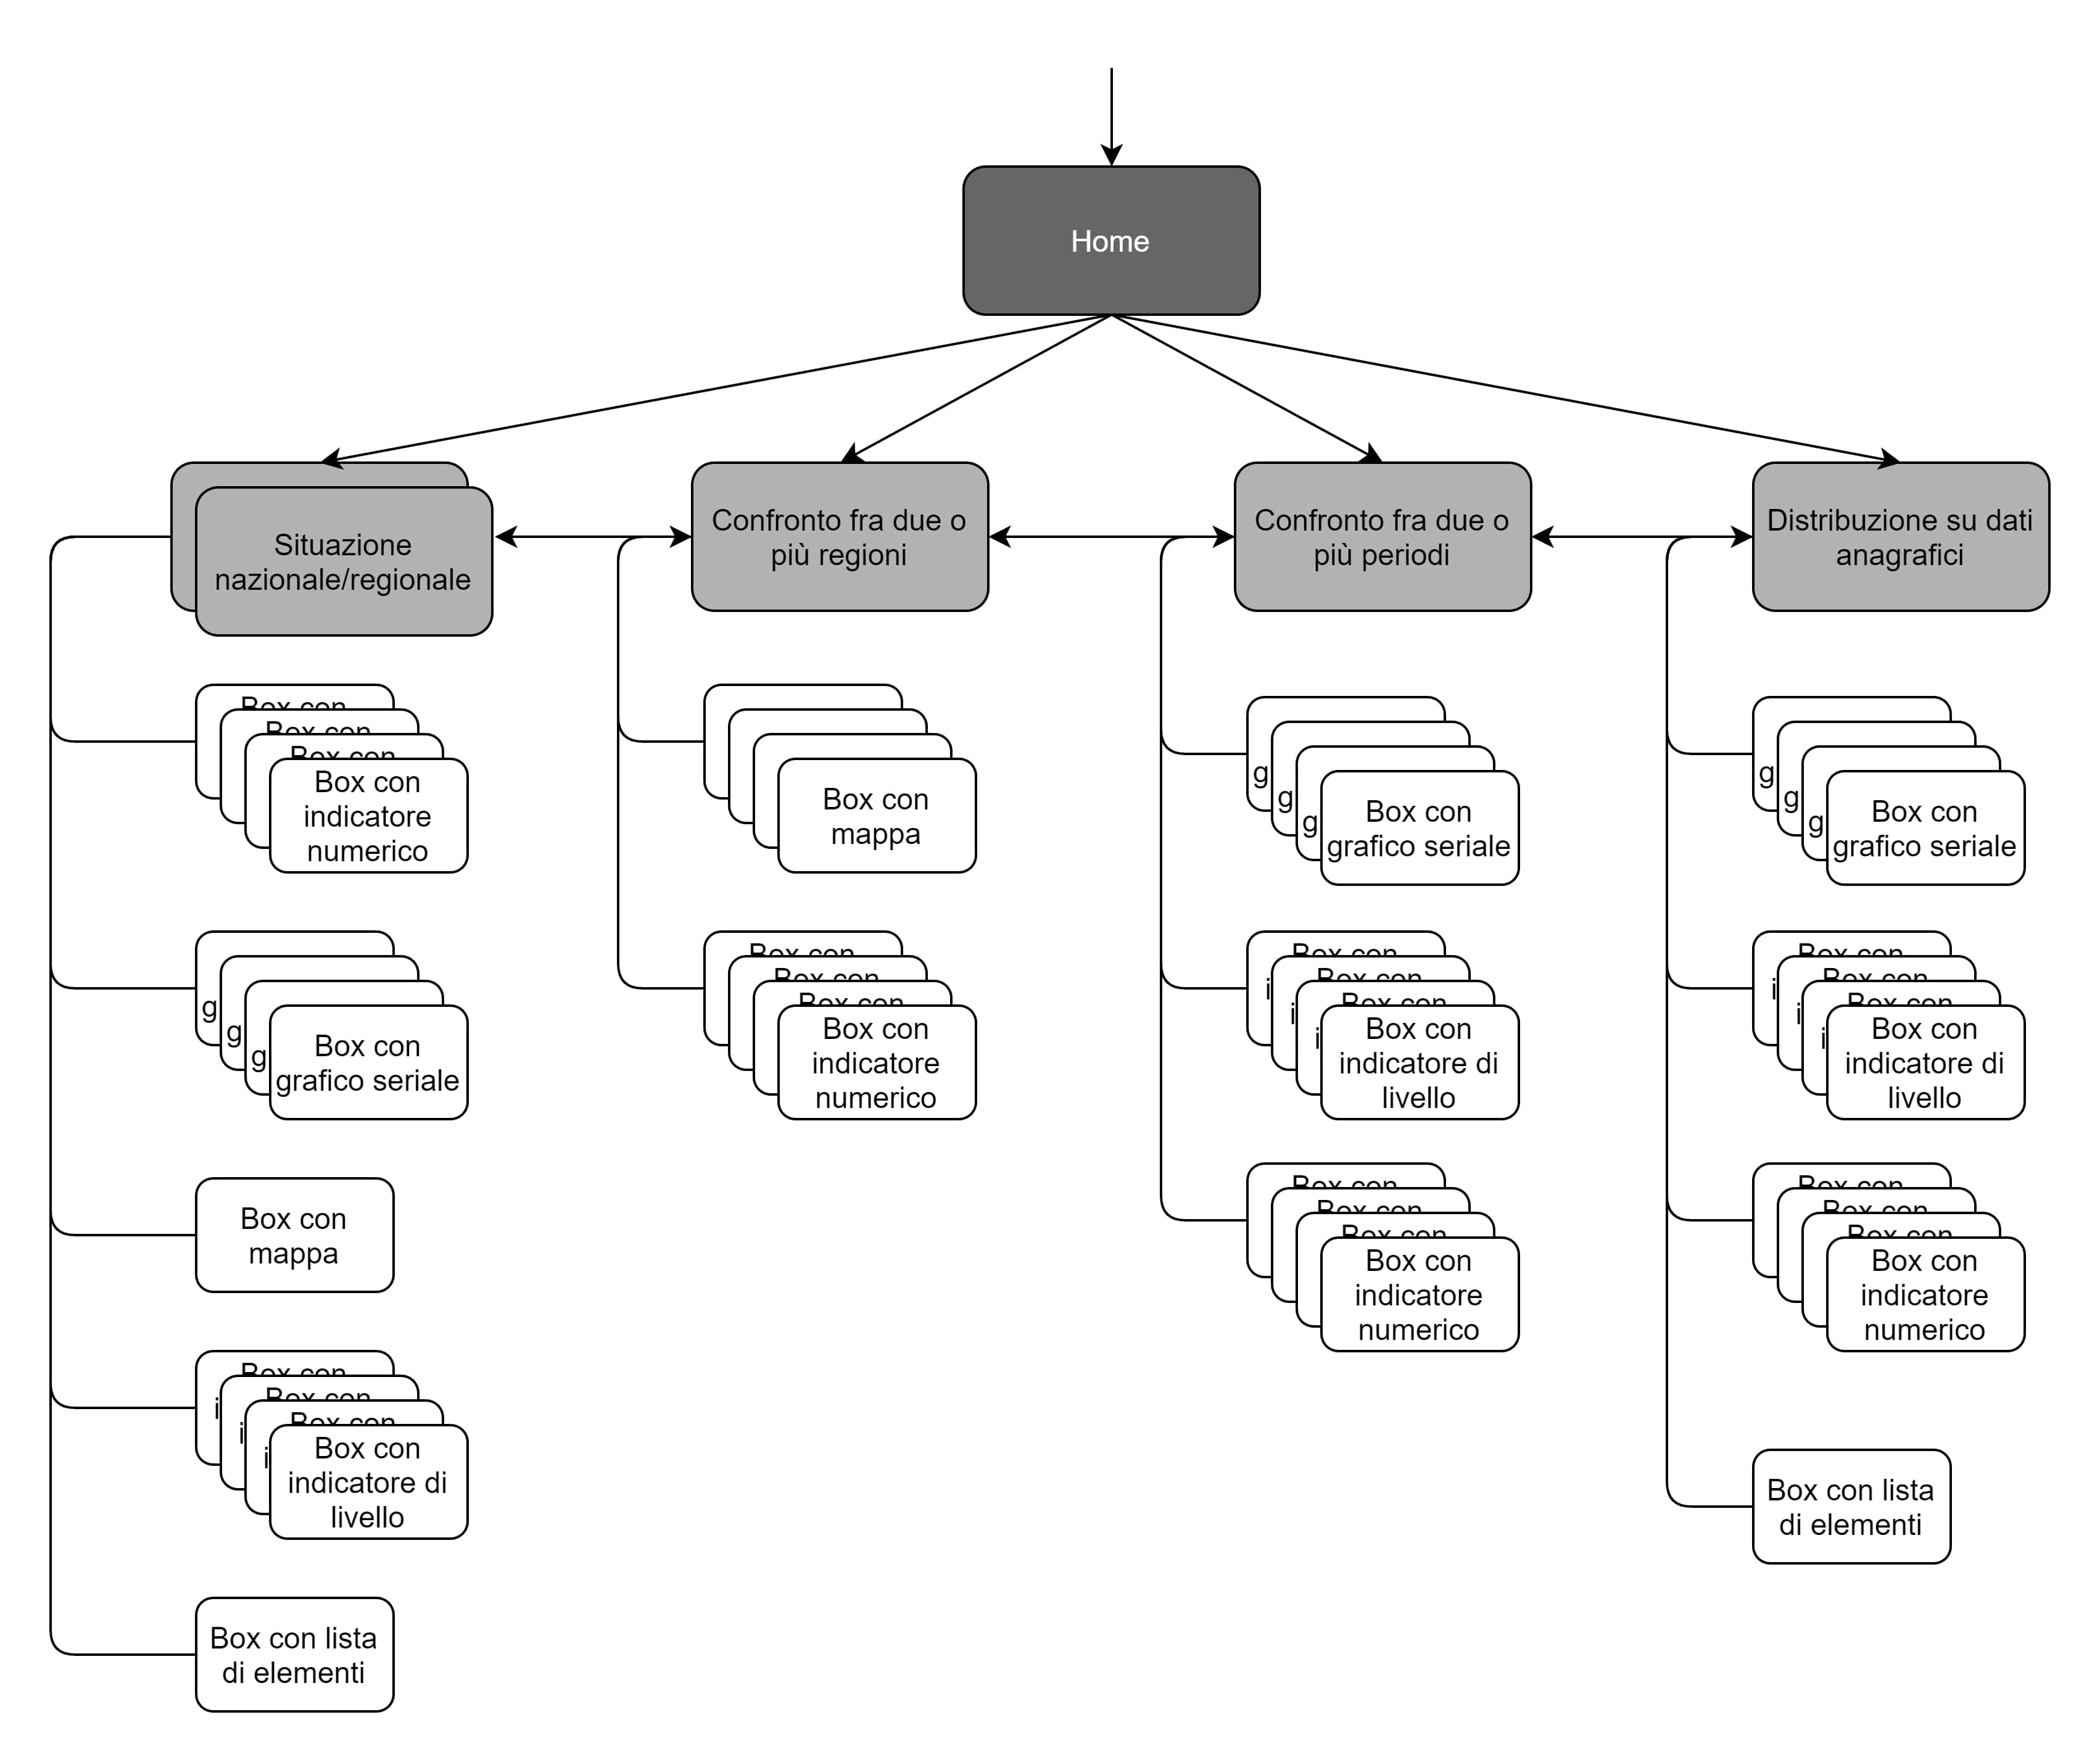
\includegraphics[width=1.0\columnwidth]{structure-blueprint/blueprint-prog-1}
    \caption{Prima versione del blueprint.}\label{fig:blueprint-prog-1}
\end{figure}
Diversamente da quanto avviene nella dashboard del DPC attuale, in principio, avevamo pensato che la home page potesse essere una semplice pagina che permettesse la scelta fra le quattro pagine indicate:
\begin{itemize}
    \item ``Situazione nazionale/regionale": due pagine simili ma con contenuto riferito l'una all'intera nazione, l'altra a una singola regione;
    \item ``Confronto fra due o più regioni";
    \item ``Confronto fra due o più periodi";
    \item ``Distribuzione sui dati anagrafici".
\end{itemize}
Ci siamo immediatamente resi conto che questa articolazione sarebbe stata scarsamente pratica poiché, già all'avvio della dashboard, l'utente non avrebbe avuto il ``colpo d'occhio''. Abbiamo quindi apportato modifiche raggiungendo una seconda versione del blueprint.

\subsubsection{Seconda iterazione}\label{ss:seconda-iterazione}
\begin{figure}[H]
    \centering
    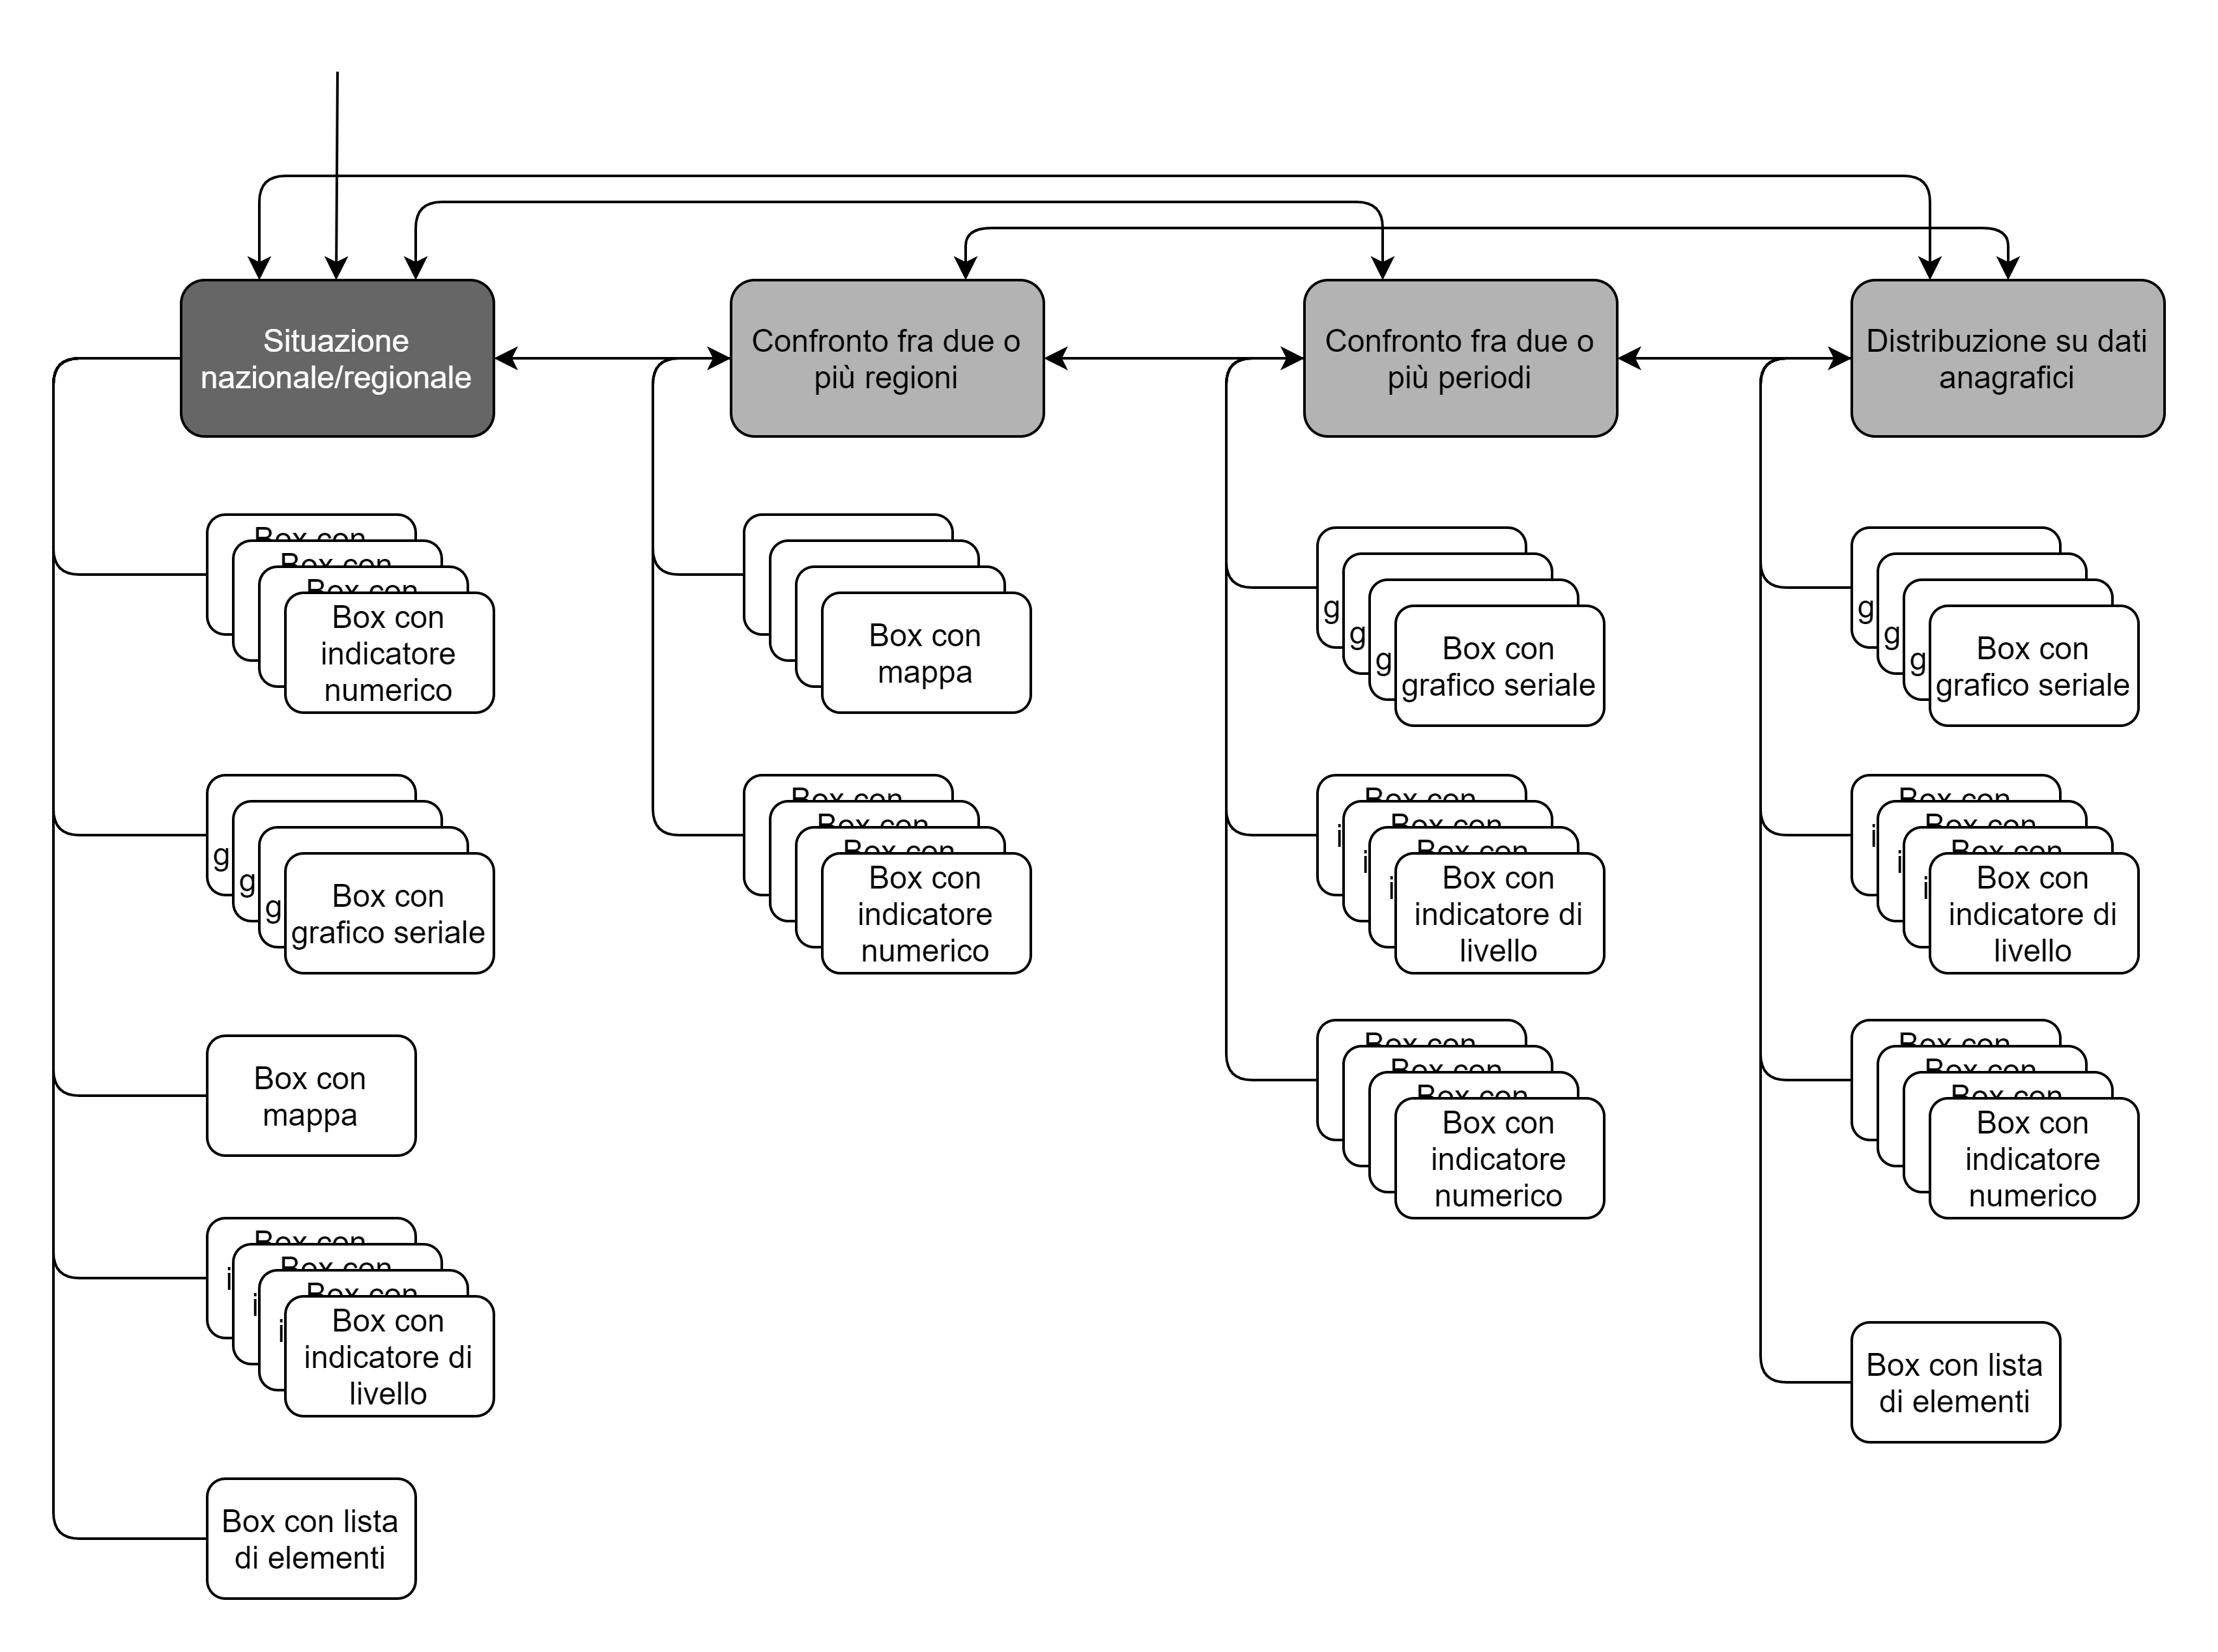
\includegraphics[width=1.0\columnwidth]{structure-blueprint/blueprint-prog-2}
    \caption{Seconda versione del blueprint per programmatori.}\label{fig:blueprint-prog-2}
\end{figure}
Questo nuovo blueprint (Figura \ref{fig:blueprint-prog-2}) mostra come la pagina principale sia ora ``Situazione odierna (nazionale/regionale)''. Le due pagine precedentemente distinte, ora, sulla scia della dashboard attuale, risultano essere la medesima: quando l'utente specifica una regione, ecco che i dati presentati sono relativi a quella regione e non più alla nazione intera, il tutto senza dover cambiare schermata.\\
\noindent
Per maggior chiarezza, abbiamo deciso di aggiungere anche un secondo blueprint (Figura \ref{fig:blueprint-cont-2}) che presenti una diversa prospettiva della struttura della dashboard: in dettaglio, il nostro focus si è spostato sul comunicare i concetti che sono presenti in ogni schermata, così da fornire una più chiara e pragmatica panoramica.
Riguardo al concetto ``Andamento giornaliero'', il livello di granularità provinciale sarà presentato all'utente solo qualora si trovi a visualizzare quel concetto a livello regionale.

\begin{figure}[H]
    \centering
    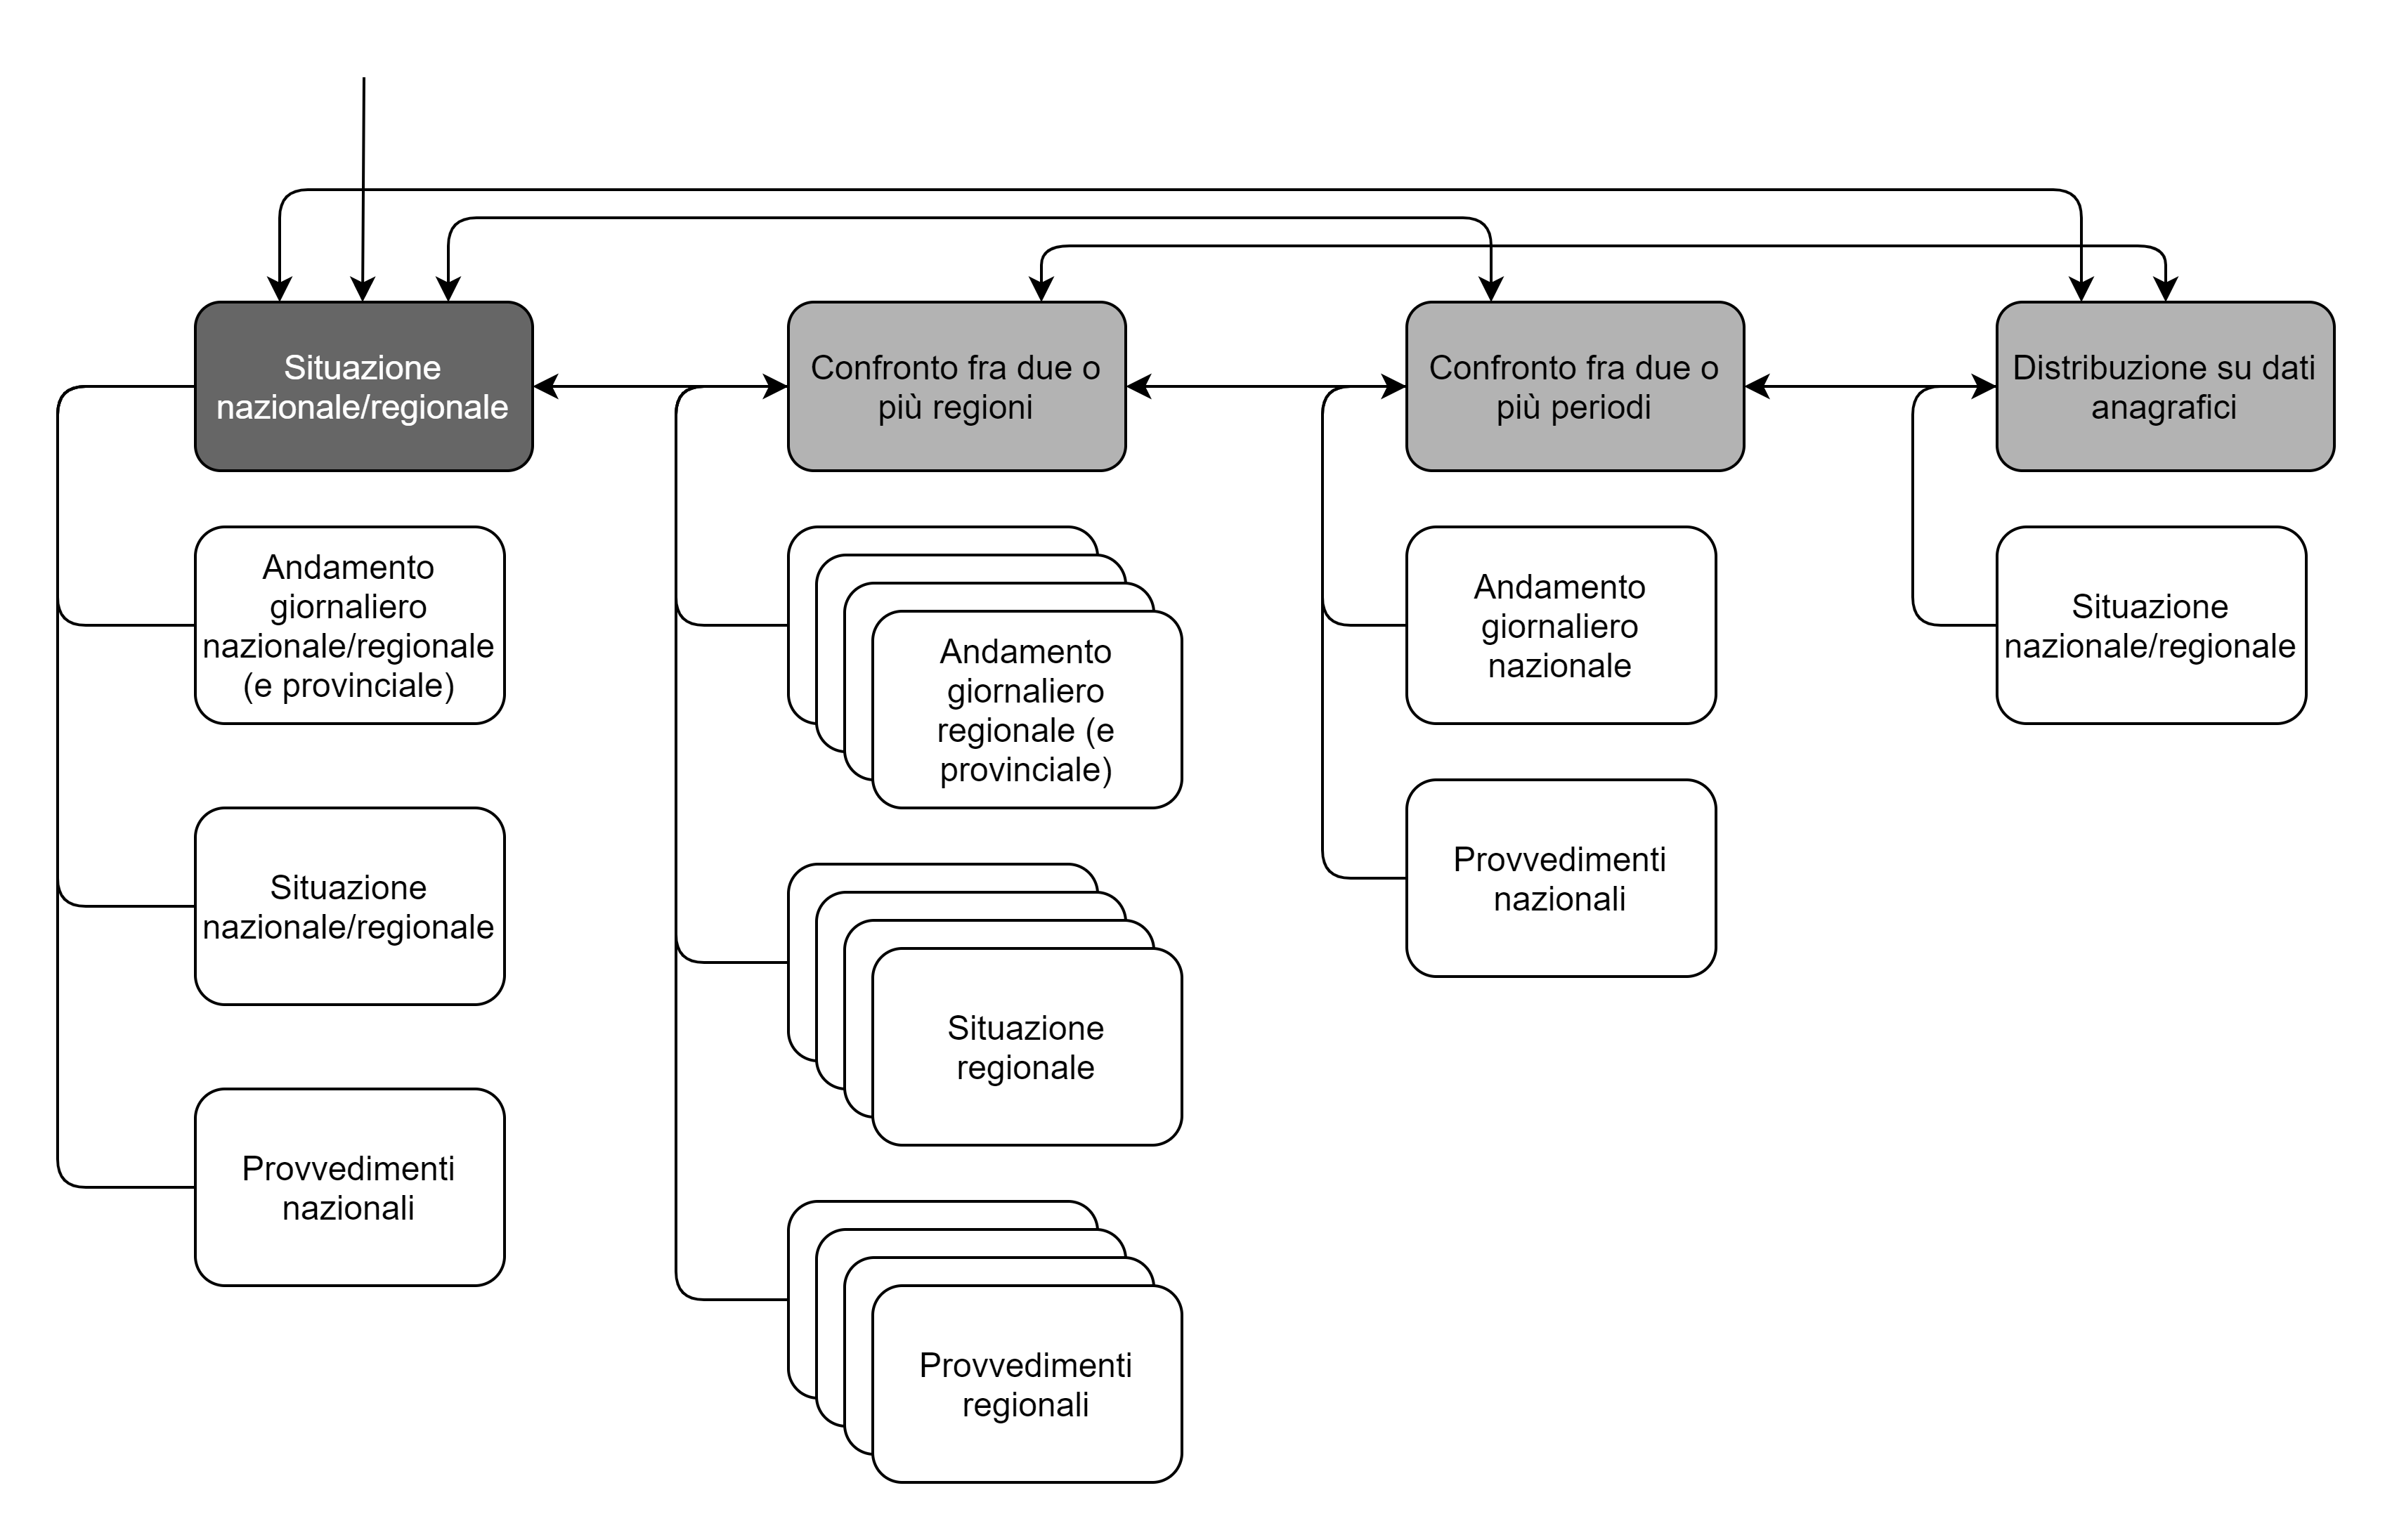
\includegraphics[width=1.0\columnwidth]{structure-blueprint/blueprint-cont-2}
    \caption{Seconda versione del blueprint per contenuti.}\label{fig:blueprint-cont-2}
\end{figure}
\clearpage
\subsubsection{Terza iterazione}
La terza iterazione ci ha portato alla realizzazione di un'ulteriore versione  dei blueprint.
\begin{figure}[H]
    \centering
    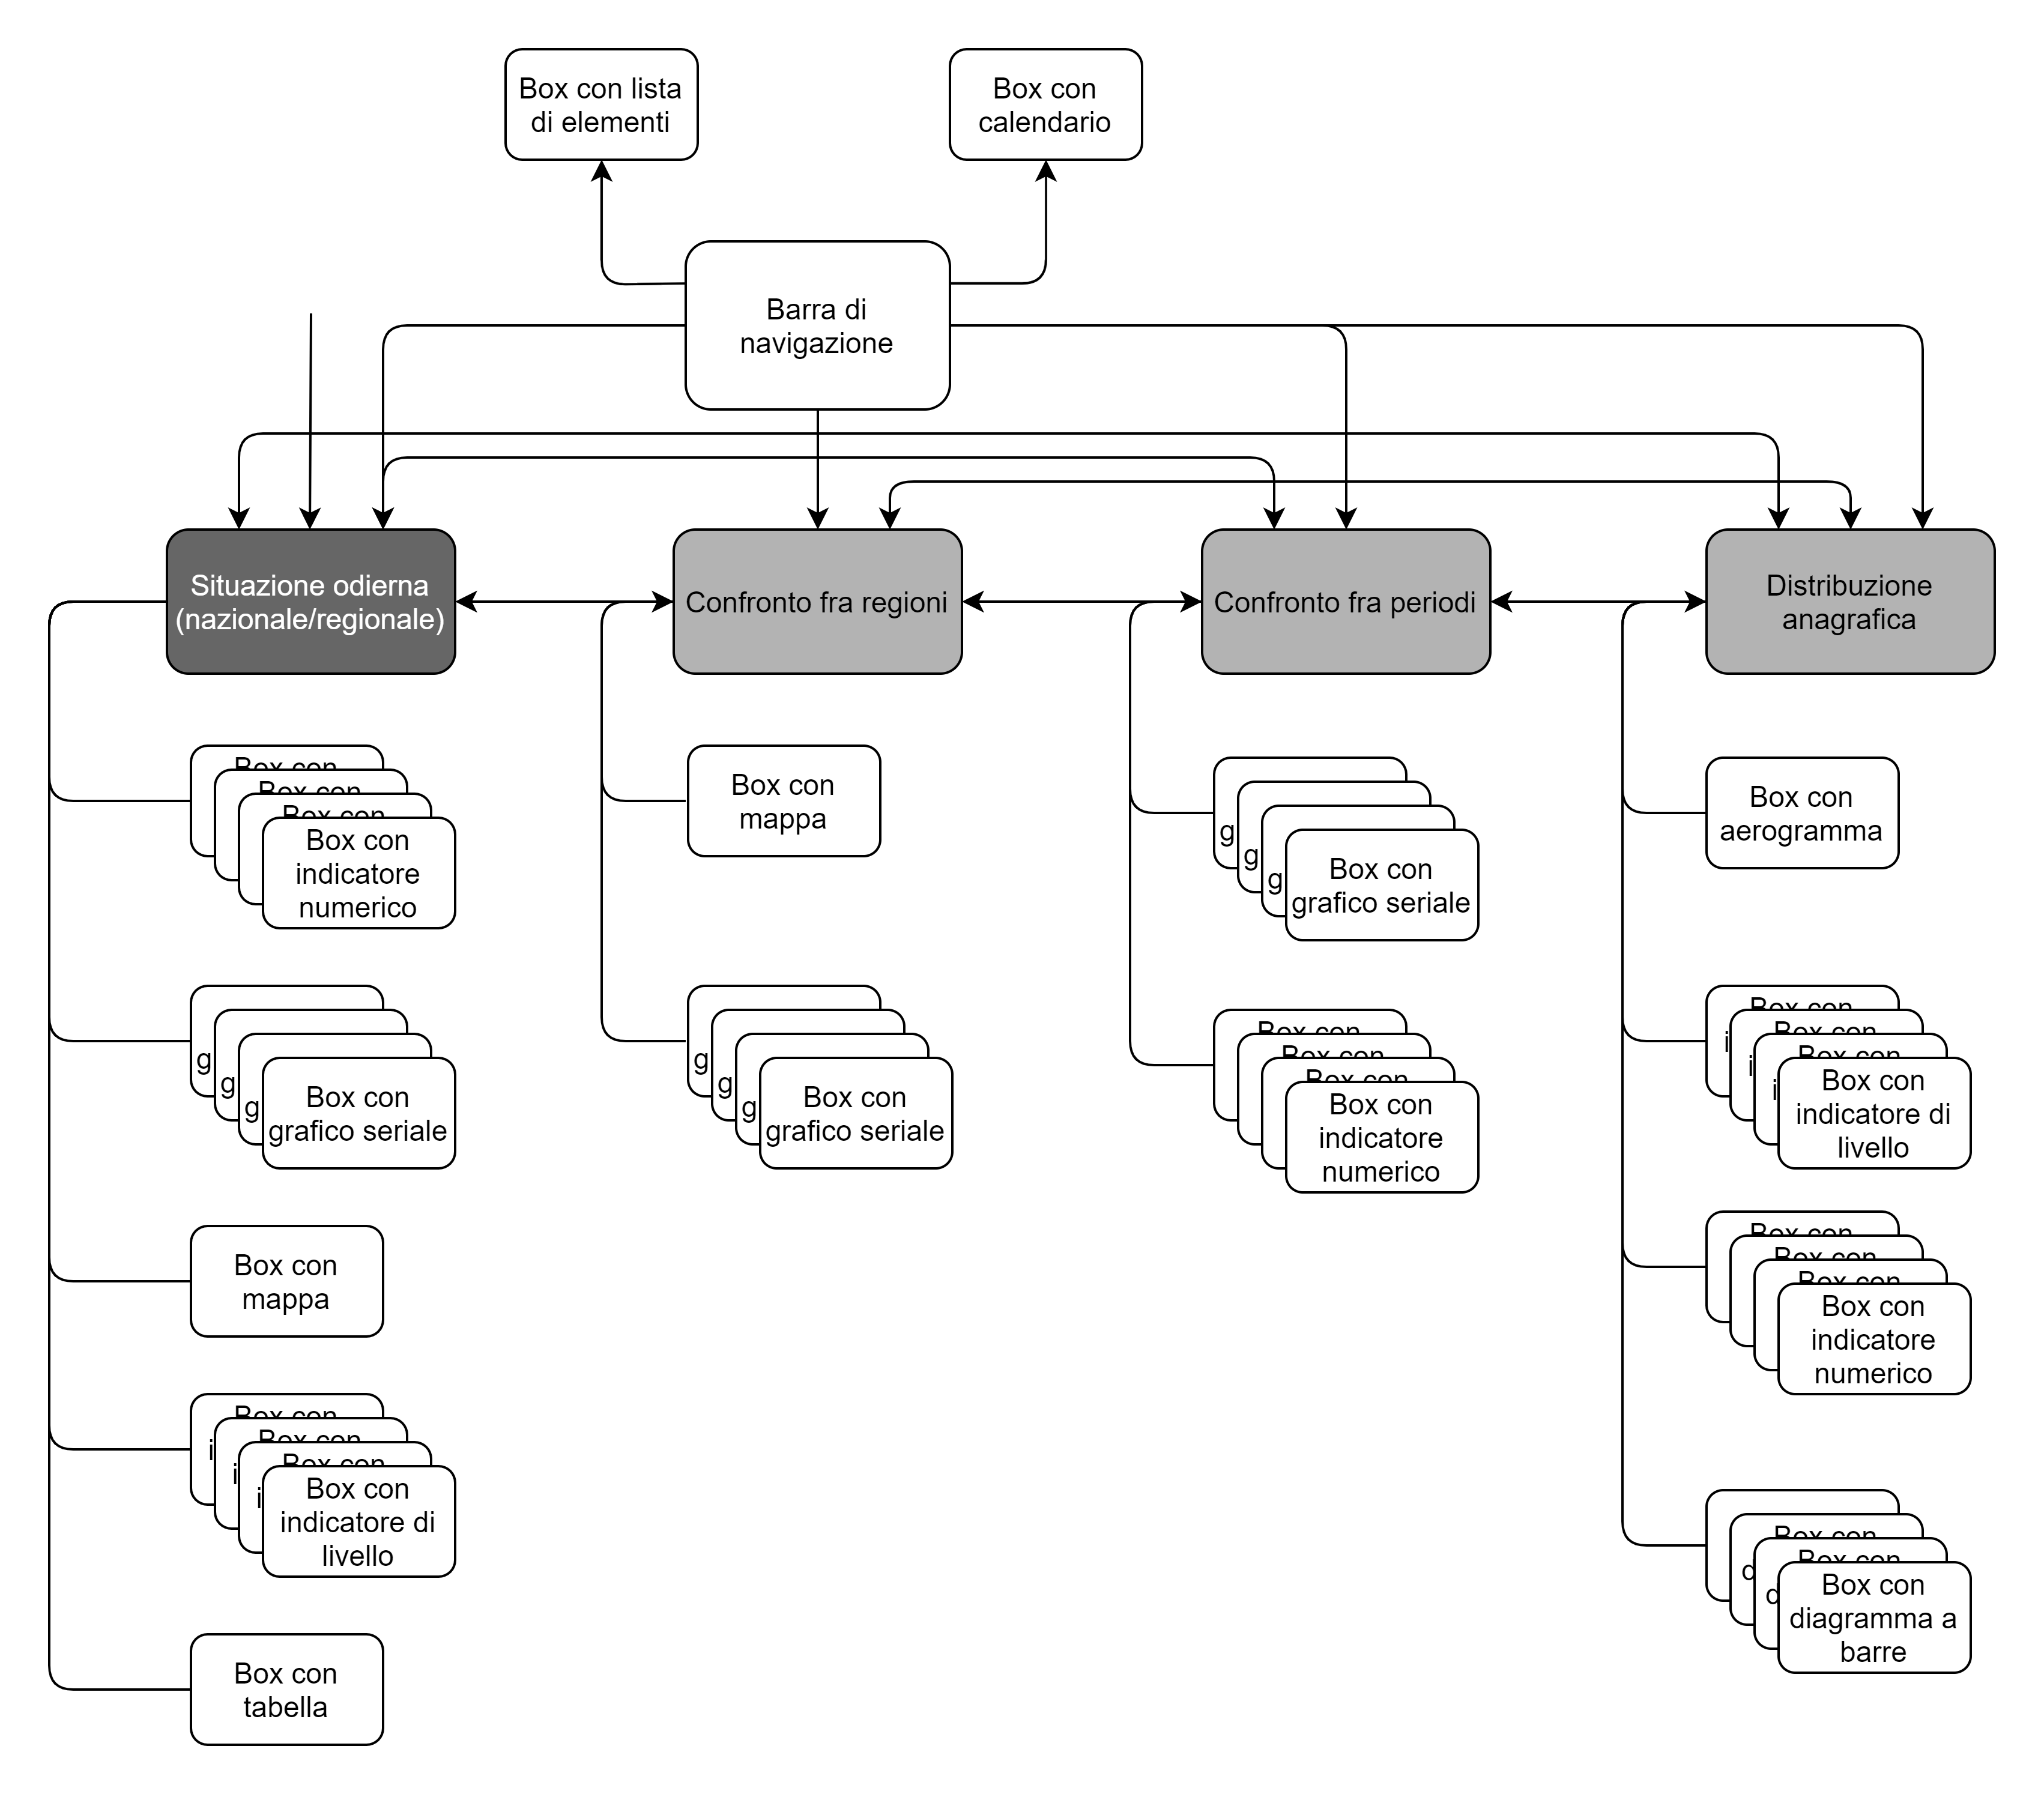
\includegraphics[width=1.0\columnwidth]{structure-blueprint/blueprint-prog-3}
    \caption{Terza versione del blueprint per programmatori.}\label{fig:blueprint-prog-3}
\end{figure}
\begin{figure}[H]
    \centering
    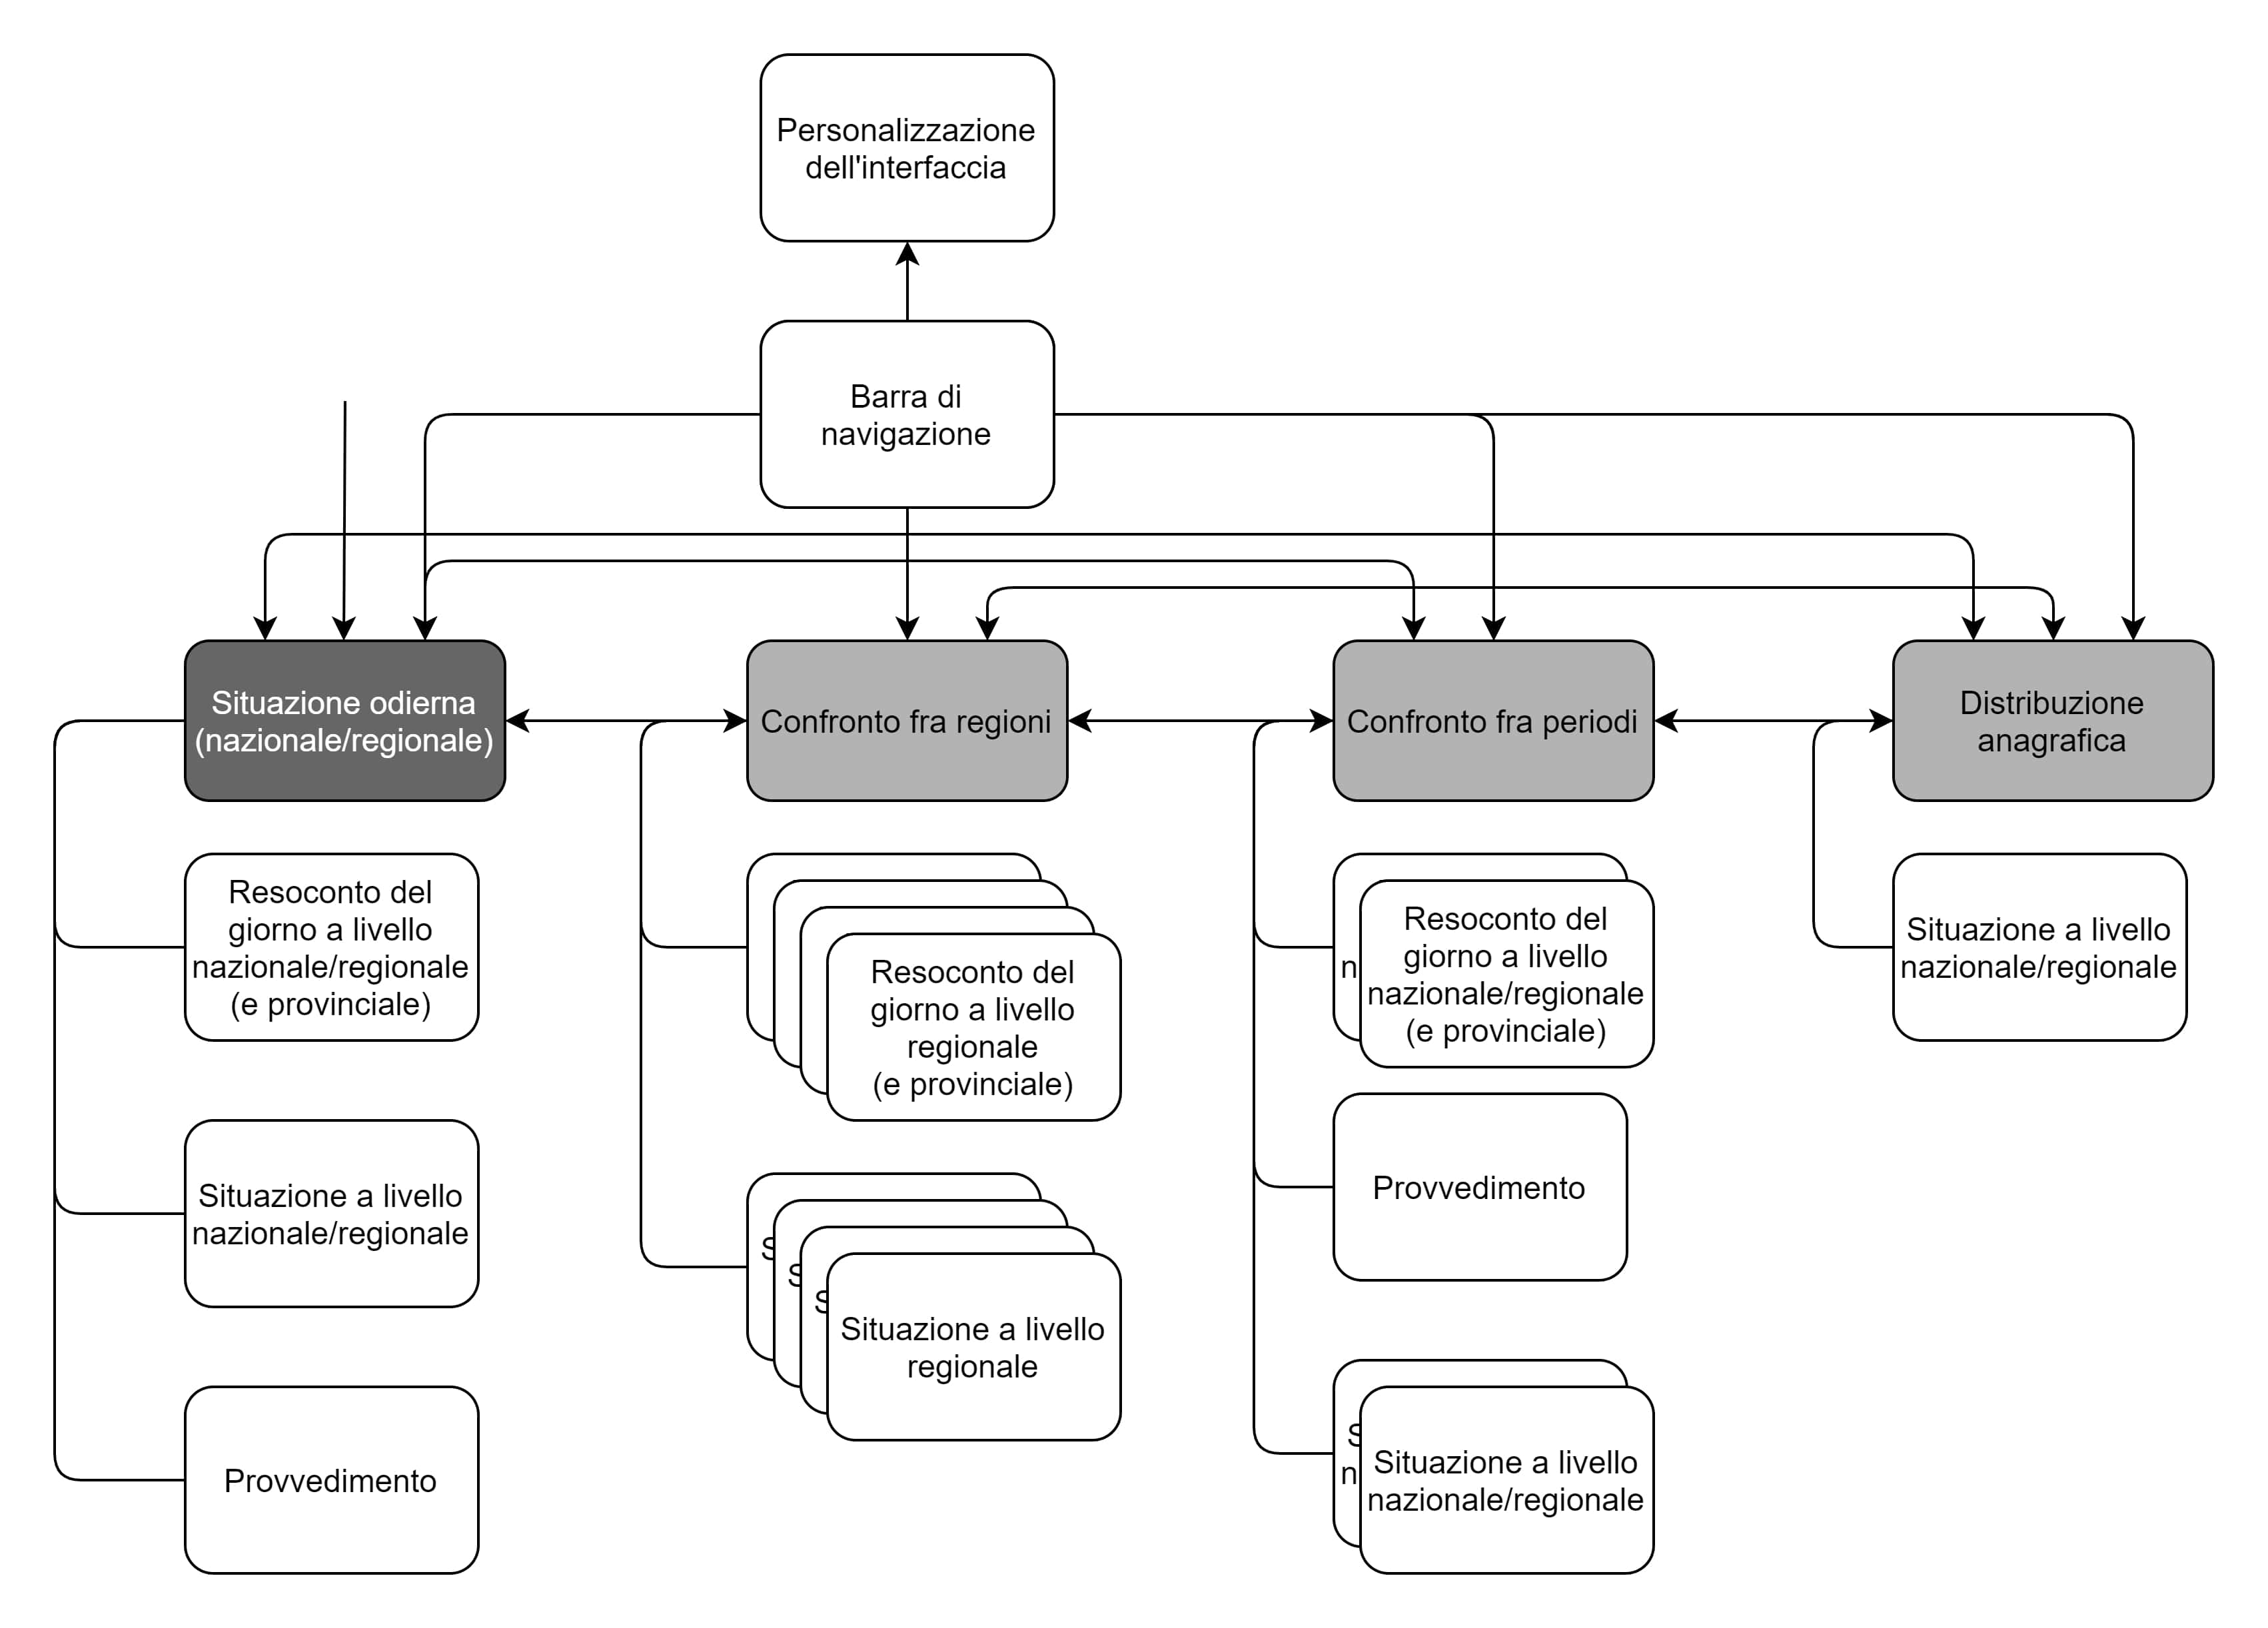
\includegraphics[width=1.0\columnwidth]{structure-blueprint/blueprint-cont-3}
    \caption{Terza versione del blueprint per contenuti.}\label{fig:blueprint-cont-3}
\end{figure}
\noindent
Durante la realizzazione dei wireframe abbiamo individuato alcune criticità nella \hyperref[ss:seconda-iterazione]{seconda versione} del blueprint; abbiamo quindi apportato alcune modifiche per risolvere le problematiche individuate:
\begin{itemize}
    \item abbiamo aggiunto un ``Box con calendario'' apribile mediante un bottone nella barra di navigazione;
    \item abbiamo aggiunto un ``Box con tabella'' in ``Situazione odierna'' per poter visualizzare in maniera più completa le metriche divise per regioni;
    \item abbiamo sostituito ``Box con indicatore numerico'' con  ``Box con grafico seriale'' in ``Confronto tra regioni'' per rendere più chiare le differenze tra le regioni che si vogliono analizzare;
    \item abbiamo eliminato il ``Box con indicatore di livello'' da ``Confronto tra periodi'' perché ritenuti poco opportuni;
    \item abbiamo aggiunto ``Box con areogramma'' e ``Box con diagramma a barre'' in ``Distribuzione anagrafica'' perché riteniamo siano particolarmente efficaci nel descrivere la distribuzione delle metriche.
\end{itemize}
Ancora, ci siamo ricordati del concetto ``Personalizzazione dell'interfaccia'', il quale nelle nostre intenzioni deve essere accessibile e attivabile da qualsiasi pagina, per cui lo abbiamo integrato nell'intestazione dell'interfaccia comune a tutte le schermate.
Inoltre, approssimandoci all'implementazione della dashboard, crediamo sia significativa una composizione di due task già definiti, quali il ``Confronto tra due o più periodi'' e il ``Confronto tra due o più regioni'': vogliamo che il giornalista possa filtrare i dati tanto relativamente alla dimensione temporale, quanto a quella spaziale, così da riuscire a confrontare l'andamento tra due o più regioni, in due o più periodi.
Infine, abbiamo rinominato ``Andamento giornaliero'' con ``Resoconto del giorno'' in ``Situazione odierna'' perché riteniamo quest'ultima espressione più chiara. 

\subsubsection{Quarta iterazione}
\begin{figure}[H]
    \centering
    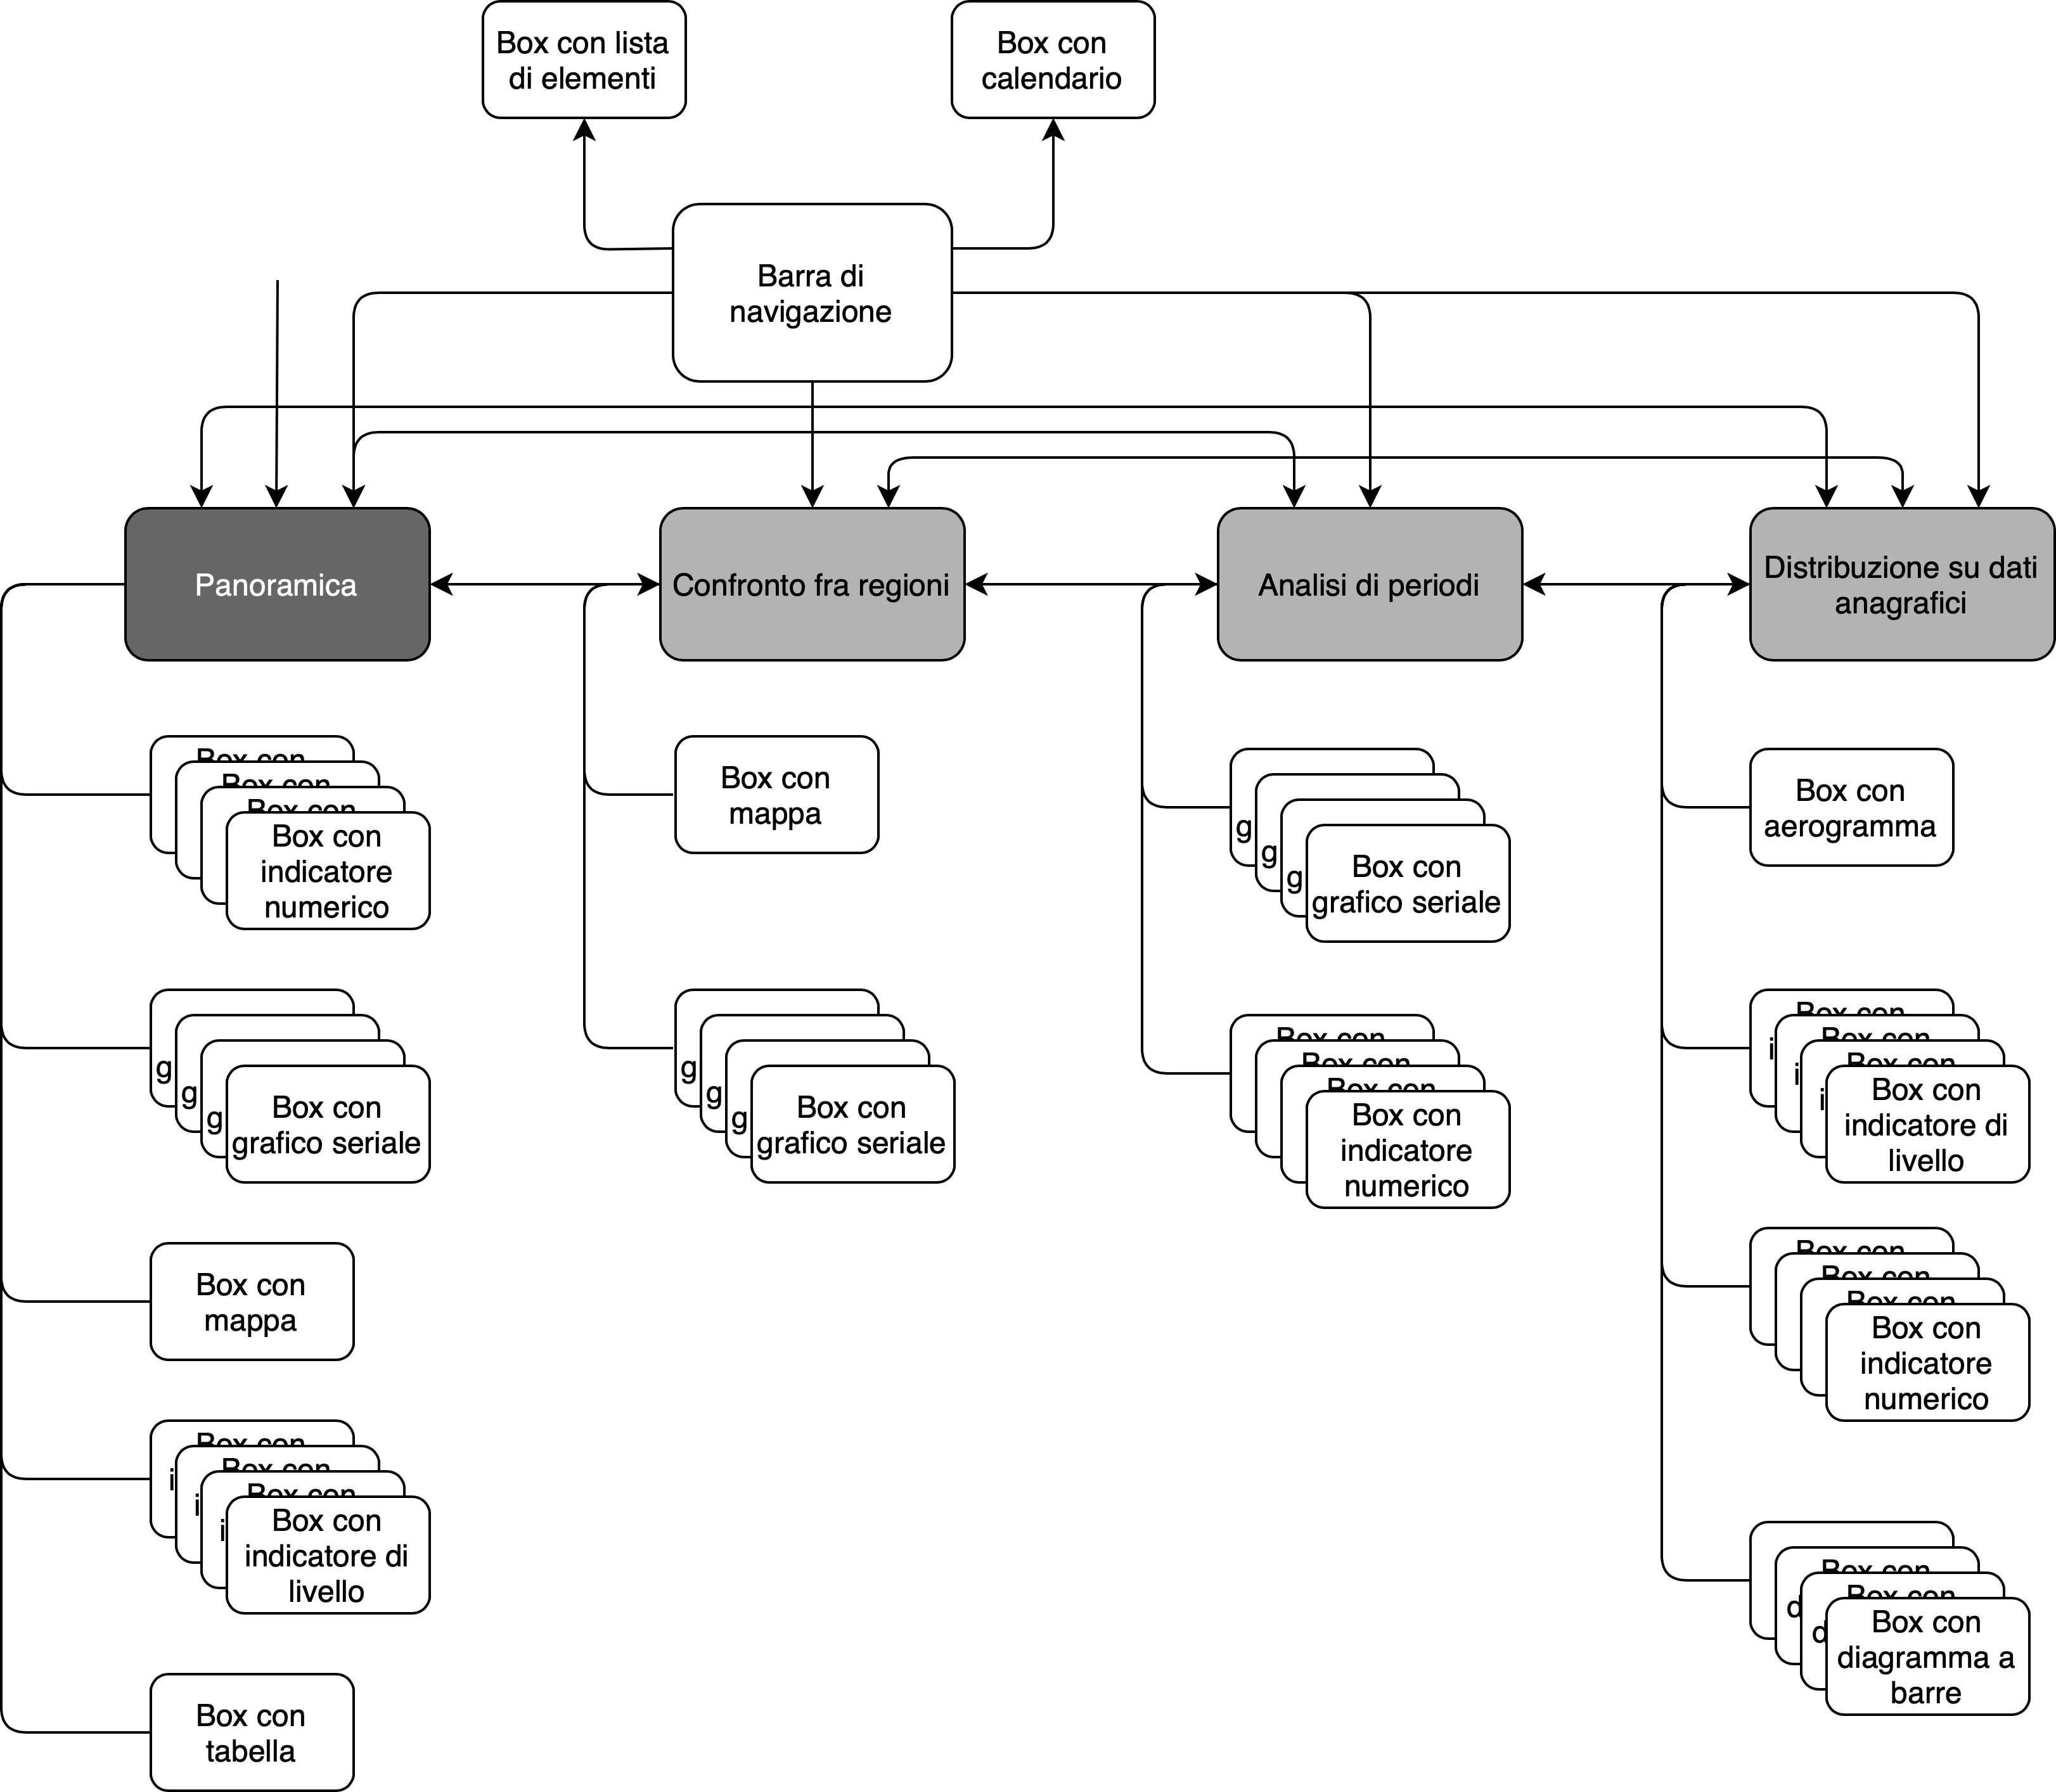
\includegraphics[width=1.0\columnwidth]{structure-blueprint/blueprint-prog-4}
    \caption{Quarta versione del blueprint per programmatori.}\label{fig:blueprint-prog-4}
\end{figure}
\begin{figure}[H]
    \centering
    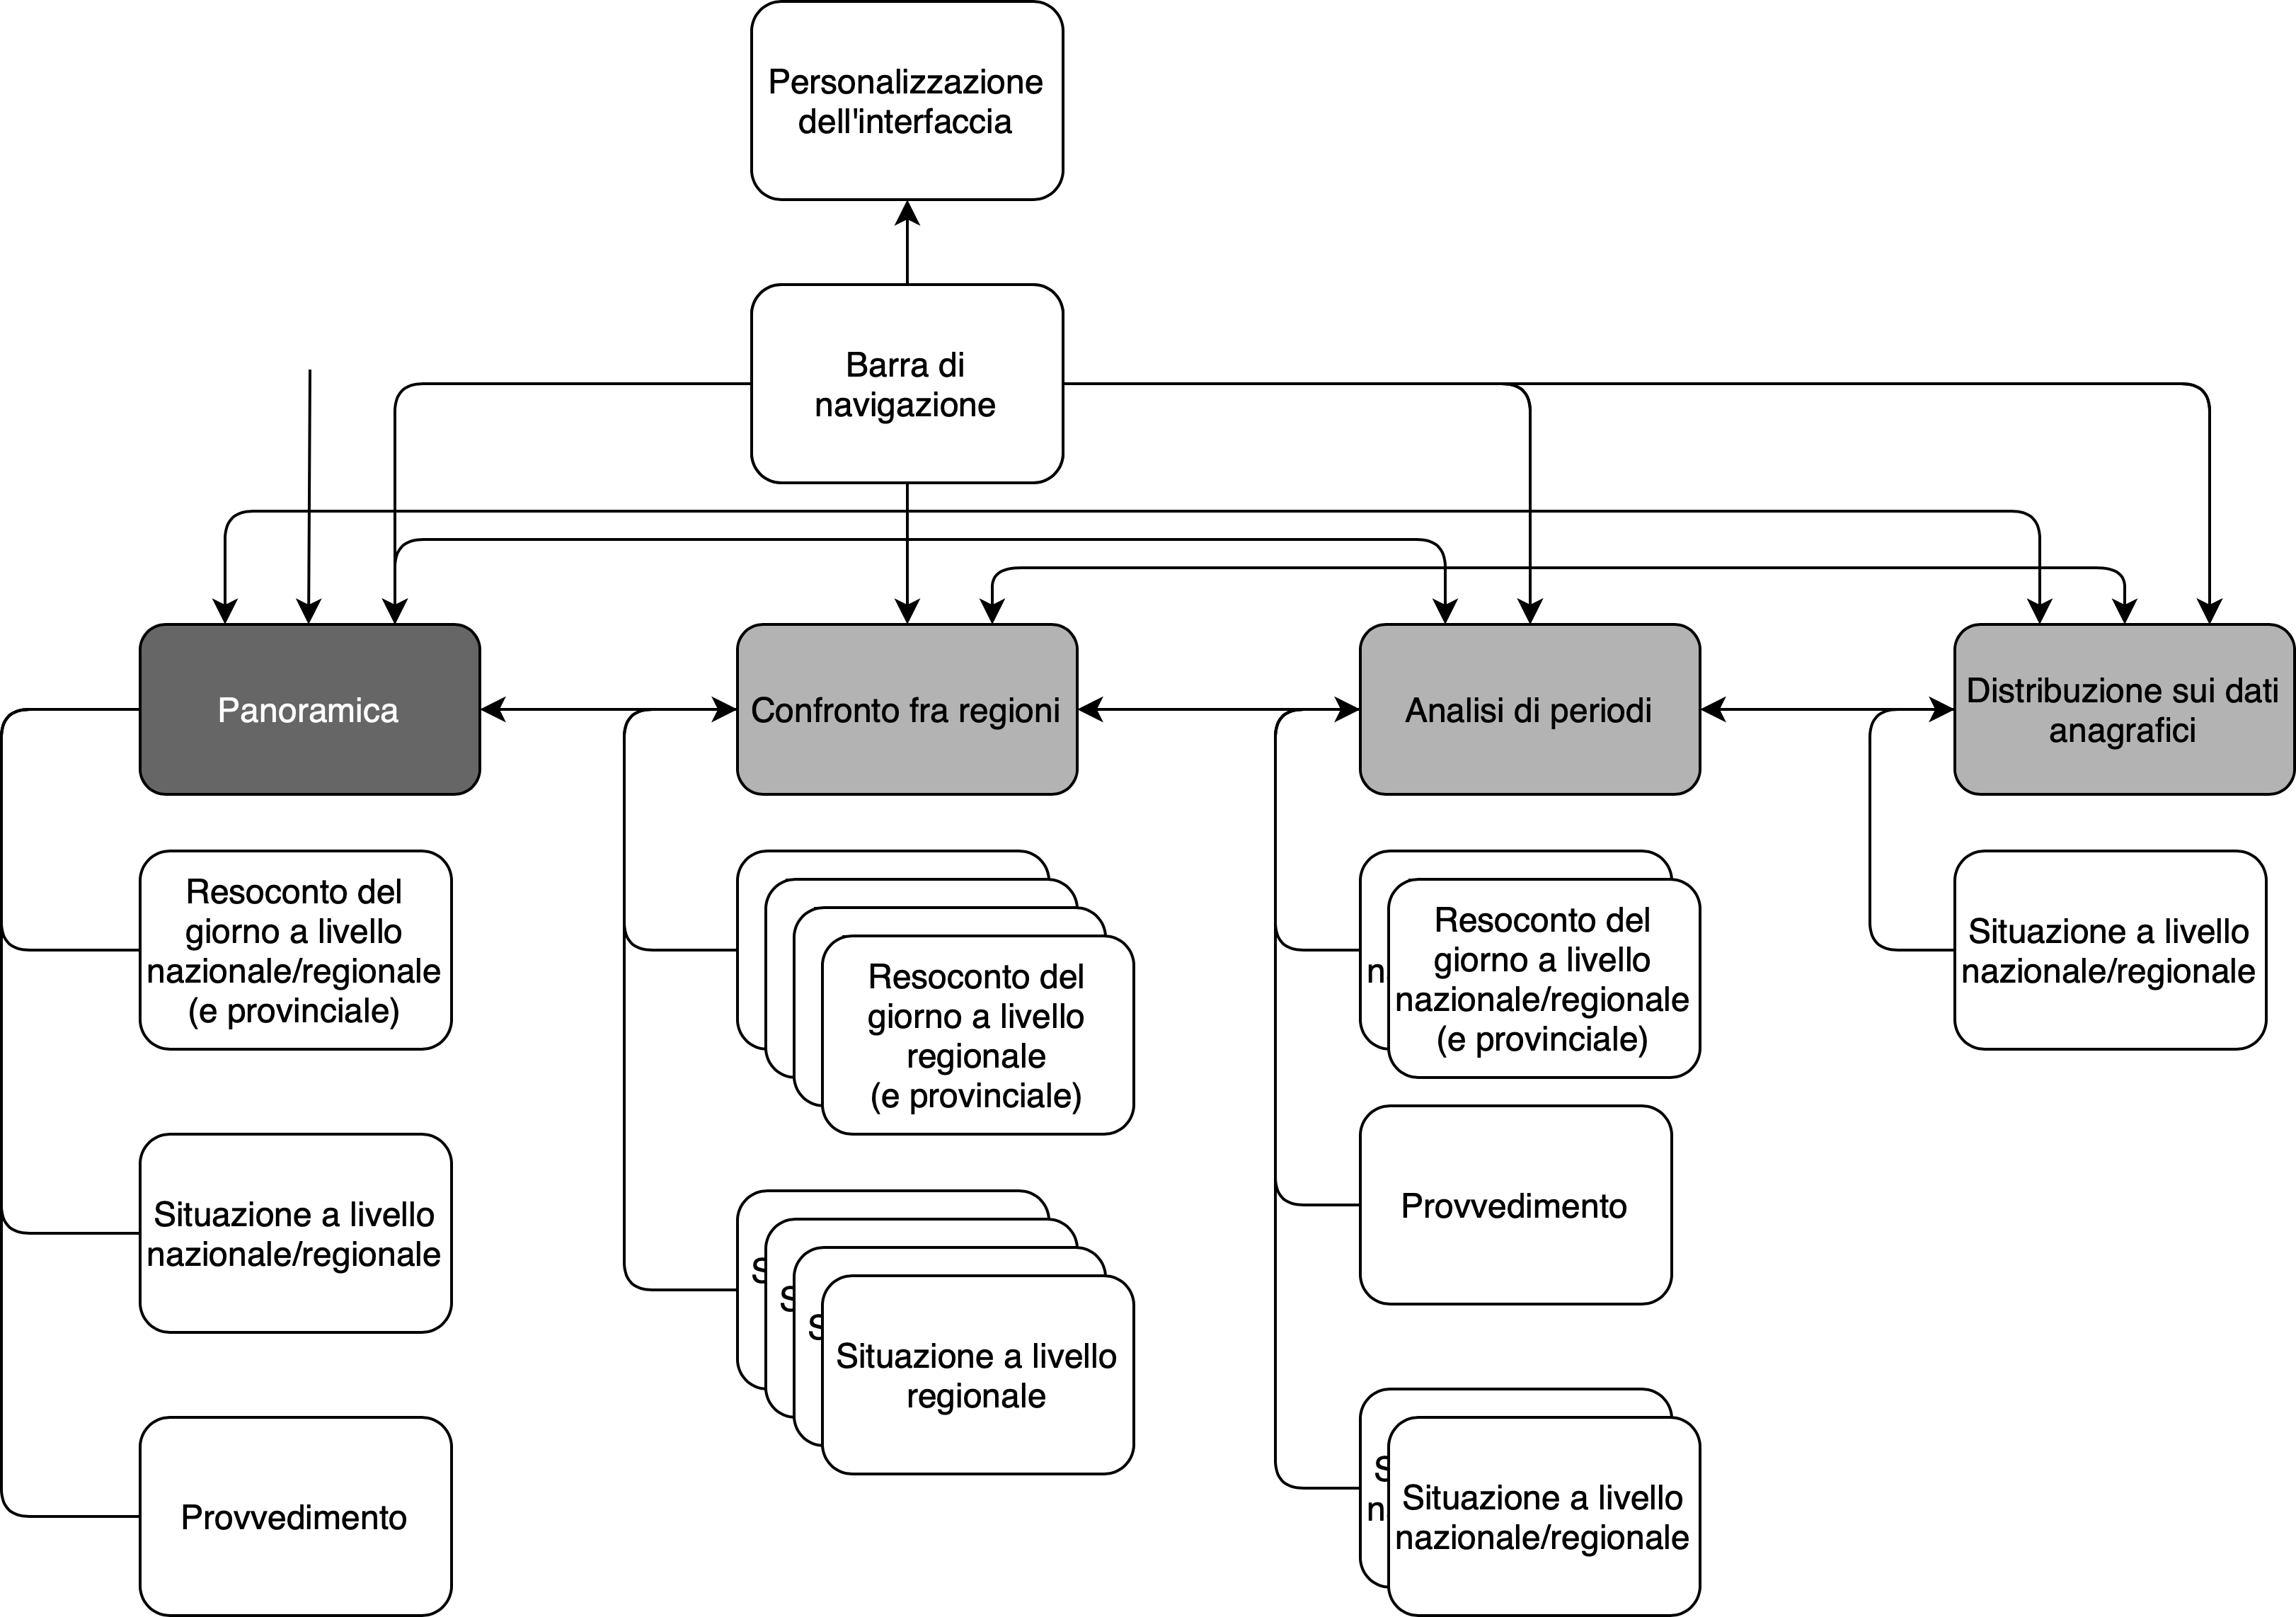
\includegraphics[width=1.0\columnwidth]{structure-blueprint/blueprint-cont-4}
    \caption{Quarta versione del blueprint per contenuti.}\label{fig:blueprint-cont-4}
\end{figure}
Successivamente a quanto svolto in \hyperref[ss:informal-action-analysis]{Sezione 5.1.2 Informal Task Analysis} abbiamo rinominato il nome delle schermate per aiutare maggiormente l'utente a comprendere cosa può fare in ogni schermata.
\begin{itemize}
    \item ``Situazione odierna'' diventa ``Panoramica'' per dissociare la schermata dal giorno odierno in quanto è possibile cambiarlo;
    \item ``Confronto fra periodi'' diventa ``Analisi di periodi'' siccome in questa schermata è possibile analizzare uno o due periodi;
    \item ``Distribuzione anagrafica'' diventa ``Distribuzione su dati anagrafici'' per rendere più chiaro il contenuto.
\end{itemize}

